\documentclass[11pt]{article}
\usepackage[includeheadfoot, top=1.0in, bottom=1.0in, hmargin=1.0in]{geometry}
\usepackage[utf8]{inputenc}
\usepackage{fancyhdr}
\usepackage{url}
\pagestyle{fancy}
\usepackage{setspace}
\usepackage{tabularx}
\usepackage{graphicx}
\usepackage{caption}
\usepackage{subcaption}
\usepackage{hyperref}
\usepackage{multicol}
\usepackage{amsmath}
\usepackage{enumitem}

\usepackage{hyperref}
\hypersetup{
    colorlinks=true,
    linkcolor=blue,
    filecolor=magenta,      
    urlcolor=blue,
}


\lhead{Astronomy Lab II}
\rhead{Spring 2023}
\lfoot{Mead \& Golant}
\rfoot{Tues 7-10pm}
\cfoot{\thepage}

\begin{document}

\begin{center}
\huge{Lab 7: Exoplanets}\\ \medskip \Large{March 21, 2023}
\end{center}

%%%%%%%%%%%%%%%%%%%%%%% INTRO %%%%%%%%%%%%%%%%%%%%%%%
\section{Introduction}

%%%%%%%%%%%%%%%%%%%%%%% TRANSITS %%%%%%%%%%%%%%%%%%%%%%%
\section{Transits: Cosmic Photobombs}

\medskip \noindent
These graphs are the \textit{only} information we get about a transiting planet. But, as simple as they are, we can learn a lot about a planet from them!  \textbf{Answer the following questions in your lab notebook:}

\begin{enumerate}
    \item \textcolor{blue}{8 pts} What happens to the depth of the ``dip" as the size of the planet gets larger (assume you are looking at the same star)? What would happen to the depth of the ``dip" if instead the size of the planet remained the same, but the star got larger?  Why?
    \textcolor{red}{The depth of the dip indicates the fraction of light from the star that is blocked by the planet.  If the planet were to get larger, fractionally, more light would be blocked.  If the star were to get larger, then the fraction of light blocked would decrease.}
    
    \item \textcolor{blue}{7 pts} Your friend says, ``You can use the transit method to measure the size of a planet without knowing the size of the star." Is your friend right or wrong? Why? What do you think you \textit{can} measure about sizes with the light curve?
    \textcolor{red}{Friend is wrong. The transit method relies on the fraction of light blocked by the planet.  If we don't know the size of the star, or how much light it puts out, then there is no way to know how big the planet has to be to block that much light.  We can measure the ratio of sizes only.}
    
    \item \textcolor{blue}{4 pts} What happens if a star has planets but their orbits are “tilted” away from us? Would we detect these planets via their transits? \textcolor{red}{No, we can only see the dip in the light curve if the planet passes directly between us and the stars along our line-of-sight.  If it is out of the plane, it would not block starlight from our perspective.}
    
    \item \textcolor{blue}{4 pts} You want to measure the \textit{period} of a planet (the time it takes for a planet to complete one lap around its star). Using the transit method, what data would you need in order to do this? \textcolor{red}{You would need multiple transits.  The time between dips would tell you how often the planet passes in front of its star, and thus, the period.}
    
\end{enumerate}

\subsection{Your Very Own Transit}
\noindent
\textcolor{blue}{14 pts}
\textcolor{red}{
\begin{enumerate}
    \item \textcolor{blue}{3 pts} Includes data table with 8 measurements with and without planet
    \item \textcolor{blue}{1 pt} Drops highest and lowest measurement of each, averages data
    \item \textcolor{blue}{1 pt} Circumference of star recorded
    \item \textcolor{blue}{3 pts} Depth of transit
    \item \textcolor{blue}{3 pts} Radius of star, area of star
    \item \textcolor{blue}{3 pts} Planet area, planet radius
\end{enumerate}}

\begin{enumerate}[label=Step \arabic*:]
    \item Have at least one member download an app which can use your phone’s camera to measure brightness (Android users, I recommend Light Meter Free; Apple users, I recommend LUX Light Meter Free). Plenty of these apps exist for photographers, but make sure you get one which uses your phone’s camera, not its light meter.
    
    \item Get a paper towel roll, or roll up/tape a piece of paper into a similar shape, then move to someplace in the room where when looking through the tube you can isolate a single one of the weird orb overhead lights (ideally one of the lower ones). This will be your target ``star"!
    
    \item Pick one of the styrofoam balls, which will be your ``planet" to detect.
    
    \item Have one member hold the tube over their camera’s lens so that just the ``star" is in view. Then, take 8 measurements of the brightness of the star. We do this since no measurement is perfect, and these apps can be finicky- real issues astronomers face with telescopes too! Write down each of your measurements in your lab notebook.
    
    \item Now, with another member standing on a stool within reach of the star, have them hold the “planet” in front of light. Take another 8 measurements, trying to change as little about the scene as possible between readings, recording these as well.
    
    \item Before stepping down, use a string and a yard stick or a flexible tape measure to record the circumference of your ``star" (the distance around the widest part).
\end{enumerate}

\noindent
Congratulations, you’ve just taken a transit measurement! Now comes the scientific analysis, let’s see what we can learn about this “planet”. First, some data science. 
\begin{enumerate}[label=Step \arabic*:,resume]
    \item Start by throwing out the highest and lowest measurements in both of your data sets, then take the average of the remaining 6 in each.
\end{enumerate}

\medskip \noindent
Now, some math! Transit analysis pivots around measuring how much light was blocked by your star. We can “normalize” the amount of light we measured by calling the out-of-transit measurements 100\%. To measure the influence of the planet:
\begin{enumerate}[label=Step \arabic*:,resume]
    \item Divide your ``with planet" average by your ``without planet" average.  Let's call this number d.  The \textit{depth} of the transit is 1 - d.
\end{enumerate}

\noindent
You might have guessed that the depth of the transit depends on the area we see of the star and the area we see of the planet. With some rearrangement, we can use our measurement of the star’s size and the transit’s depth to get a measurement of the planet’s size! First, we need to calculate the area of your star.

\begin{enumerate}[label=Step \arabic*:,resume]
    \item Using the circumference, C, that you measured for your star, calculate the radius, R (\textit{hint: }$R = \frac{C}{2\pi}$).
    \item The area of a circle (which is how a star appears to us on the sky) is $A = \pi R^2$.  Solve for the area, A, of your star.
\end{enumerate}

\medskip \noindent
Now we can combine that area and the measured depth into an estimate of the planet's size. The planet can be thought of as ``negative area" when it's in front of the star, something which blocks a small patch we would have otherwise seen. 
\begin{enumerate}[label=Step \arabic*:,resume]
    \item Multiply your transit depth by the area of your star -- this is the area your planet blocks, while it transits, or in other words, the area of your planet!

    $$\text{Planet Area} = (\text{1 - d}) \times \text{A}$$
    
    \item Using this area, solve for the radius of your planet (\textit{hint: }rearrange the equation for A from step 10) This is your measured planet radius! Now, measure the circumference of your planet and calculate its radius the same way you did with your star in step 9.

\end{enumerate}


\medskip \noindent
Some final things to consider:
\begin{enumerate}
\setcounter{enumi}{4}
    \item \textcolor{blue}{4 pts} Is the radius you derived from brightness measurements similar to the one you actually measured when holding the planet? If not, do you have any ideas for why that might be? \textcolor{red}{Probably not. Sources of error include: poor quality of the app, shifting of distance between observer and ``star", funnel was too large and let in other light, or changed size.}
\end{enumerate}


%%%%%%%%%%%%%%%%%%%%%%% RV %%%%%%%%%%%%%%%%%%%%%%%
\section{Wadial Wobbles: The Radial Velocity Method}
\subsection{Predictions} \label{sec:RV_predictions}

\begin{enumerate}
\setcounter{enumi}{5}
    \item \textcolor{blue}{3 pts} Check out this gif from the Wikipedia page on radial velocity: \url{https://en.wikipedia.org/wiki/Radial_velocity#/media/File:Planet_reflex_200.gif}.  You'll notice that both planet and star orbit around a common \textit{center of mass}, but this point is generally still inside the star itself.  Make a generalized statement that describes how the star moves relative to the planet. Or in other words, where is the star in its orbit at each point of the planet's orbit?
    \textcolor{red}{The planet and star are always at opposite points in their orbits. That is, as the star is moving toward us, the planet is moving away and vice versa.}
        
    \item Assume that we on Earth are viewing this system edge on from the bottom of the gif.
        \begin{enumerate}
            \item \textcolor{blue}{3 pts} When the planet is moving away from us on Earth (on the left side of the gif), would the star's light be redshifted or blueshifted? What about when the planet is moving towards us (on the right side of the gif)? \textcolor{red}{Blueshifted, then redshifted.  Star is moving oppositely to the planet so towards then away from us.}
            
            \item \textcolor{blue}{3 pts} When the planet is directly in front of or behind the star, will we see any spectral shift? (\textit{Hint}: Think about whether there is any motion \textit{towards} or \textit{away} from us at these points.) \textcolor{red}{No, there is no motion towards or away from the observer.}
        \end{enumerate}
        
    \item Let's think about how our orientation relative to the star-planet system affects our ability to take radial velocity measurements.
        \begin{enumerate}
            \item \textcolor{blue}{3 pts} We know that if we view the system edge on ($90^\circ$ inclination), as above, we can see the spectrum shifting because there is motion towards or away from us.  If we slowly decrease the inclination towards a face-on system ($0^\circ$ inclination), would we get more or less shifting of the spectral lines? Why? \textcolor{red}{We would get less shifting of the spectral lines because there is less motion towards and away from us.}
            
            \item \textcolor{blue}{3 pts} If we were viewing a system face-on, would we be able to tell there is a planet using radial velocities? Why or why not? \textcolor{red}{No, all of the motion is perpendicular to us, there is no motion towards or away from us at all.}
        \end{enumerate}
        
    \item Finally, let's make some predictions about how a system's properties affect the radial velocity of the star.
    \begin{enumerate}
        \item \textcolor{blue}{3 pts} Holding the \textit{planet} mass constant, if we increase the star's mass, will the star have higher or lower radial velocity? Why? \textcolor{red}{Lower RV, it is harder for the planet to tug, the relative gravitational influence from the planet is smaller.}

        \item \textcolor{blue}{3 pts} Holding the \textit{star} mass constant, if we increase the planet's mass, will the star have higher or lower radial velocity? Why? \textcolor{red}{Higher RV, the planet has more mass and will exert a stronger gravitational tug on the star.}

        \item \textcolor{blue}{3 pts} Holding the \textit{star and planet} mass constant, if we increase the semimajor axis of planet (distance from the star), will the star have higher or lower radial velocity? Why? \textcolor{red}{Lower, as the planet moves further from the star, it's gravitational influence will be smaller, so it will exert a smaller tug on the star.}

    \end{enumerate}
        
\end{enumerate}

\subsection{RV Simulator}
\noindent
If you haven't already, you should download the appropriate ``NAAP Labs" package from \url{https://astro.unl.edu/nativeapps/} for your machine.  Once you have installed it, open the application on your computer.  Under ``Extrasolar Planets", select ``Exoplanet Radial Velocity Simulator".  This should open another window with the simulator.  If you are having technical trouble with this, let me know.

\medskip \noindent
\textbf{In your lab notebooks, set up a table with columns to record measurements for the quantity/quantities you are testing, and a description column.}  In the ``Description" column, I want you to 1) record the amplitude of the radial velocity of the star, and 2) describe the shape of the RV curve.

\begin{enumerate}
\setcounter{enumi}{9}
    \item \textcolor{blue}{7 pts} First, write a brief description of how you will test your prediction.  What quantities will you vary and why? \textcolor{red}{Grade for reasoning}
    \item \textcolor{blue}{3 pts} Using the Option A preset, make a few ``observations" by varying your chosen property/ properties.  Record your findings in your table. \textcolor{red}{Table}
    \item \textcolor{blue}{4 pts} Describe the trend you found during your exploration. Does this trend match your prediction from Section \ref{sec:RV_predictions}?  If not, why? \textcolor{red}{Grade for reasoning}

    \item \textcolor{blue}{1 pt} Consult with your group about their findings before moving on.  Were your predictions correct, and if not, why not? \textcolor{red}{Grade for completion}
    
    \item \textcolor{red}{Not done}
    
    \item \textcolor{red}{Not done}
    
    \item \textcolor{red}{Not done}
    % Edge on
\end{enumerate}

\section{A Plethora of Planets}
Go to the NASA Exoplanet Archive plotting tool (\url{https://exoplanetarchive.ipac.caltech.edu/cgi-bin/IcePlotter/nph-icePlotInit?mode=demo&set=confirmed}).  Plot each of the following, and then write a few sentences on what you learn from each plot (what trends do you observe, what do you think they mean, what do large empty spaces on the plot mean/why are observations bias towards the sample that is plotted).  Use what you now know about the transit and RV methods. \textit{Hint:} Kepler's 3rd law states that the period of a planet's orbit squared is directly proportional to the distance between the star and the planet cubed ($P^2 \propto a^3$). \textbf{Include your plots in your lab write-up.}  \textcolor{red}{3 pts for trend, 4 pts for bias, 3 pts for interpretation, 1 pt for graph}
    \begin{enumerate}
    \setcounter{enumi}{16}
        \item \textcolor{blue}{11 pts} Planet Radius (x-axis) vs. Orbital Period (y-axis). \textcolor{red}{Grade on reasoning. Trend appears to be flat.  Most detected planets have radii within and OoM of Jupiter and short periods under 100 days.  This is likely because large planets are easiest to detect (block the most light) and short periods make it easy to do multiple observations. There are very few detections for small radius planets because the amount of light they block is small and the dip is indistinguishable from noise. Long period planets take too long to detect and we are less likely to catch them. Together, small planets that are far away from their stars are less likely to transit as angles get large far away from where they are measured from.  Very short period planets (less than 1 day orbit) are uncommon as they would have to be extremely close to the star.}
        \item \textcolor{blue}{11 pts} Planet Mass (x-axis) vs. Orbital Period (y-axis).  \textcolor{red}{Grade on reasoning.  Trend broadens at high mass - this is because with a large planet, we can get further away from the star and still detect it using RV.  We don't see small, long period planets because they exert negligible gravitational influence.}

    \end{enumerate}


%%%%%%%%%%%%%%%%%%%%%%% CONCLUSIONS %%%%%%%%%%%%%%%%%%%%%%%
\section{Wrapping Things Up}

\begin{figure}[h!]
    \centering
    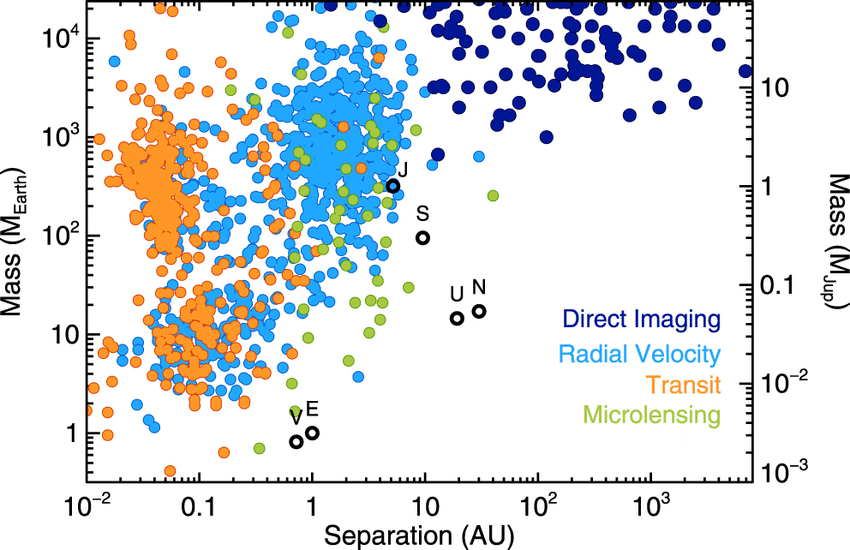
\includegraphics[width=0.8\textwidth]{Images/Exoplanet Demographic Techniques.png}
    \caption{Demographics of exoplanets colored by detection techniques. Credit: Bowler, 2016.}
    \label{fig:techniques}
\end{figure}

\begin{enumerate}
\setcounter{enumi}{18}
    \item Figure \ref{fig:techniques} is a plot of the masses of discovered exoplanets versus their distance from their host stars, colored by the detection method that was used to discover them. Let's think about why certain methods may be biased towards detecting certain types of planets.
    \begin{enumerate}
        \item \textcolor{blue}{4 pts} Using what you learned in this lab, explain why planets detected with the transit technique are (a) primarily massive and (b) close to their host stars. \textcolor{red}{Massive stars are generally also large so will block lots of light.  The closer planets are to their stars, the easier it is to capture one in transit (short period, geometrically more likely to transit even if there is a small tilt).}
        \item Using this same plot, we see that we can detect planets using the radial velocity method out to larger separations.
        \begin{enumerate}
            \item \textcolor{blue}{4 pts} Why are we able to use the RV method to detect planets further away from their hosts than the transit method? \textcolor{red}{Planets still exert gravitational influence but far away from the star are geometrically less likely to transit.}
            \item \textcolor{blue}{4 pts} Why can't we detect small planets far away from their stars using the RV method? \textcolor{red}{Small planets and far away planets exert small gravitational tugs on their stars.  This goes doubly for a small and distant planet.}
        \end{enumerate}
    \end{enumerate}
\end{enumerate}


\end{document}